\documentclass[letterpaper,10pt]{article}

\usepackage{titling}
\usepackage{listings}
\usepackage{url}
\usepackage{setspace}
\usepackage{subfig}
\usepackage{sectsty}
\usepackage{pdfpages}
\usepackage{colortbl}
\usepackage{multirow}
\usepackage{multicol}
\usepackage{relsize}
\usepackage{amsmath}
\usepackage{fancyvrb}
\usepackage{amsmath,amssymb,amsthm,graphicx,xspace}
\usepackage[titlenotnumbered,noend,noline]{algorithm2e}
\usepackage[compact]{titlesec}
\usepackage{XCharter}
\usepackage[T1]{fontenc}
\usepackage{tikz}
\usetikzlibrary{arrows,automata,shapes,trees,matrix,chains,scopes,positioning,calc}
\tikzstyle{block} = [rectangle, draw, fill=blue!20, 
    text width=2.5em, text centered, rounded corners, minimum height=2em]
\tikzstyle{bw} = [rectangle, draw, fill=blue!20, 
    text width=4em, text centered, rounded corners, minimum height=2em]

\newcommand{\CPP}{C\nolinebreak\hspace{-.05em}\raisebox{.4ex}{\tiny\bf +}\nolinebreak\hspace{-.10em}\raisebox{.4ex}{\tiny\bf +}}
\def\CPP{{C\nolinebreak[4]\hspace{-.05em}\raisebox{.4ex}{\tiny\bf ++}}}

\let\LaTeXtitle\title
\renewcommand{\title}[1]{\LaTeXtitle{\textsf{#1}}}


\addtolength{\oddsidemargin}{-1.000in}
\addtolength{\evensidemargin}{-0.500in}
\addtolength{\textwidth}{2.0in}
\addtolength{\topmargin}{-1.000in}
\addtolength{\textheight}{1.75in}
\addtolength{\parskip}{\baselineskip}
\setlength{\parindent}{0in}
\renewcommand{\baselinestretch}{1.5}

\singlespace

\begin{document}

\lecture{32 --- Convergence \& Ergodicity}{\term}{Jeff Zarnett}

\section*{Convergence}

Think back to calculus class. Remember when we talk about limits: $\lim_{x\to\infty} f(x)$. There is an answer for this if the function does (somehow) converge on some value, such as the function $f(x) = 1/x^{2}$ converging to 0.

We would like to see that our random variables converge. You might flip a coin four times and all four times it comes up heads. That doesn't match our expectation that we should have about half heads and half tails. We have convergence if, given enough samples and enough sample paths, it will converge to the 0.5 we expect. There may be some sample paths that don't converge (e.g., continually coming up heads), but they have a ``probability mass'' of zero (i.e., they are incredibly unlikely).  There are in fact uncountably many ``bad paths'', each with probability zero (but that's okay). Zero probability doesn't mean it can't happen, mind you.

An image of what convergence looks like~\cite{pmd}:

\begin{center}
	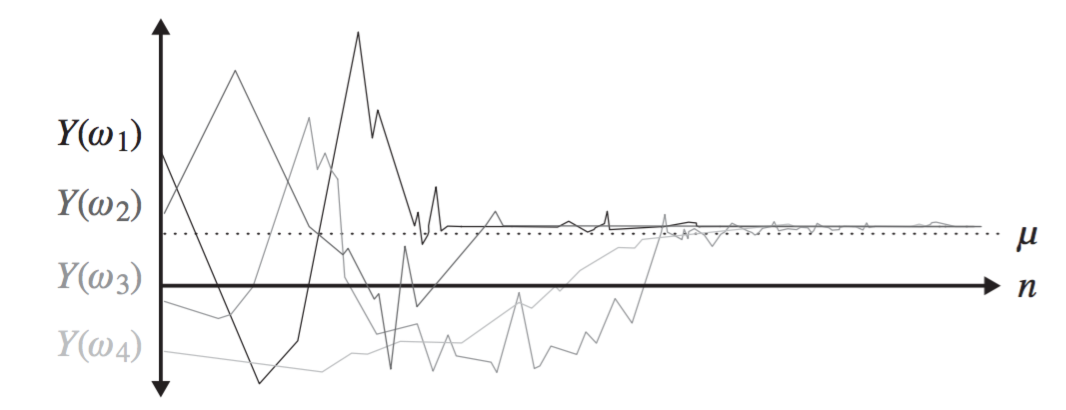
\includegraphics[width=0.6\textwidth]{images/convergence.png}
\end{center}

We won't concern ourselves with systems where there is no convergence. We'll just deal with situations where there is a convergence. Almost every sample path (series of experiments) will eventually behave well if we take enough samples. That is, get past the initial conditions. But sampling is important in our discussion about scalability...

\section*{Tim and Enzo}
A small but important digression on the subject of sampling, measurement, and testing, from~\cite{pmd}. You have an idea of what an average is, but there are two different relevant types of average here---the time average and ensemble average. 

Let us just focus on having a single First-Come-First-Serve queue. Every second, a new job arrives with probability $p$ and if there is any work to do, the job being worked on is completed with probability $q$ (and $q > p$). As a definition, let $N(v)$ equal the number of jobs in the system at a time $v$. In the story, Tim and Enzo are trying to simulate the FCFS system to determine what is the average number of jobs in the system. 

Tim decides he's going to run it as one really long simulation. He simulates the queue over a very long period, logging as he goes, taking a million samples. Then he takes the average value over those samples to get the average number of jobs.

Enzo does something slightly different: instead of having one super long simulation, he does 1000 shorter simulations. He waits until the simulation has run for 1000 seconds and then samples the queue at exactly that point, obtaining one value. This experiment is restarted with a new random seed. So after obtaining a thousand samples, he averages these, and Enzo produces another average number of jobs.

A little illustration of Tim and Enzo from~\cite{pmd}:

\begin{center}
	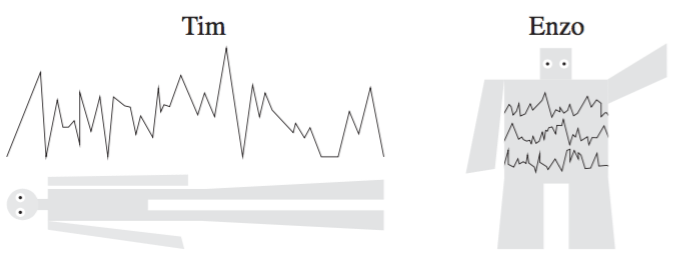
\includegraphics[width=0.5\textwidth]{images/timenzo.png}
\end{center}

So -- who has done this correctly, Tim or Enzo?

The time average has potential problems because we are only looking at a single sequence and maybe something very unusual has happened here in this single run. The ensemble average is more likely what we talk about when we talk about the system being at ``steady state'' (i.e., past the initial conditions). So we kind of like the Enzo approach. Plus, this is programming for performance (or as a student said, programming for parallelism) -- we can do 1000 simulations concurrently if we have enough CPU cores! Tim's approach still has some merit though.

A note about initial conditions: both the Tim and Enzo approaches here require caring about the initial conditions. Enzo needs to make sure that the initial conditions (startup costs etc) have attenuated before the measurement point. Tim needs to ensure that the initial conditions impact a sufficiently small portion of all his measurements.

But! If we have a nicely behaved system, the time average and the ensemble average are the same (so both Tim and Enzo can be correct). What is a nicely behaved system? The word for this is \textit{ergodic}. That probably did not help, so what is an ergodic system? It is a system that is positive recurrent, aperiodic, and irreducible.

\textit{Irreducibility} means a process should be able to get from one state to any other state (where state is the number of jobs in the system). This means the initial state of the system does not matter. So if we started at 0 jobs or 10 we could still get to any state in the system (jobs at 2 or 27)\ldots

\textit{Positive recurrence} means that given an irreducible system, any state $i$ is revisited infinitely often, and the time between visits to that state are finite. So we can define a certain state as being a ``restart''. The logical choice in the case of a queue or similar is the idea of the queue being empty. Every time the queue gets down to zero jobs, it's a ``restart'' of sorts. 

This is what makes Tim's view and Enzo's view potentially the same. A single long run (Tim's view) is just like a number of independent runs (Enzo's view). Every time we get down to zero jobs in the queue, it's a restart. 

The \textit{aperiodicity} condition is required for the ensemble average to make sense or exist. That is to say, the state of the system should not be related to the time; i.e., it is not the case that the system is in state 0 when $t$ is even and state 1 when $t$ is odd. Otherwise the way Enzo chooses to sample, i.e., $t = 1000$, is potentially going to skew the result.

A graphical illustration, also from~\cite{pmd}, that shows how the time average over a single long run can be considered a chain of restarts or ``renewals''.

\begin{center}
	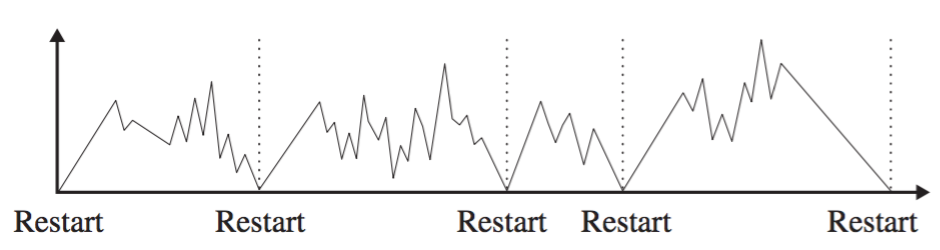
\includegraphics[width=0.5\textwidth]{images/systemrestart.png}
\end{center}

Both Tim and Enzo are correct for ergodic systems. Either method works to determine measurements and queueing theory values. Enzo's method has some advantages, e.g. parallelism and the ability to produce confidence intervals.

We've talked about the average number of jobs, but perhaps what we also care about is how long a job spends in the system, on average. We could compute either the time or ensemble average. 

\begin{center}
	Time Average = $\lim_{t\to\infty}\dfrac{\sum_{i=1}^{A(t)} T_{i}}{A(t)},$
\end{center}

where $A(t)$ is the number of arrivals by time $t$ and $T_{i}$ is the time in the system of arrival $i$. The average is taken over one sample path.

\begin{center}
	Ensemble Average = $\lim_{t\to\infty}E[T_{i}],$
\end{center}

where $E[T_{i}]$ is the average time in the system of job $i$, average being taken over all sample paths.

\bibliographystyle{alphaurl}
\bibliography{459}


\end{document}
